\documentclass[12pt]{beamer}
\usepackage{listings}
\usepackage{tabu}
\usepackage{booktabs}
\beamertemplatenavigationsymbolsempty
\AtBeginSection[]
{
    \begin{frame}
    \frametitle{Table of Contents}
    \tableofcontents[currentsection]
    \end{frame}
}
\lstset{language=C++, basicstyle=\footnotesize, frame=single}

\title{Miscellaneous math}
\subtitle{Fast pow, Fibonacci, tortoise and hare}
\author{beCP Training}
\institute{
\includegraphics[height=12em]{../share/beoi-logo}}

\begin{document}

\frame{\titlepage}

\section{Fast pow}

\begin{frame}
\frametitle{Powers}
Definition:
\begin{itemize}
\item Chain multiplication
\item ``$n$-th power of $b$''
\item $b$ is the base, $n$ is the exponent
\item $b^n = \underbrace{b\times\cdots\times b}_\text{$n$ times}$
\end{itemize}
Examples:
\begin{itemize}
\item $3^0 = 1$ (by definition)
\item $3^1 = 3$
\item $3^2 = 3 \times 3 = 9$ (square)
\item $3^3 = 3 \times 3 \times 3 = 27$ (cube)
\end{itemize}
\end{frame}

\begin{frame}[fragile]
\frametitle{Power computation: linear}
\textbf{Problem:} compute the power the $n$-th power of $b$, for given $b$ and $n$.

~

\textbf{Solution 1:} Simple loop
\begin{lstlisting}[frame=single]
int nthPower(int b, int n)
{
    int power = 1;
    for (int i = 0; i < n; i++)
        power *= b;
    return power;
}
\end{lstlisting}
Complexity: $O(n)$
\end{frame}

\begin{frame}
\frametitle{Power computation: logarithmic (1)}
Can we do it faster? Yes, because associativity!

~

For example, to compute $3^{10}$, we can compute $3^5$ then square it:
\begin{itemize}
\item $3^2 = 3 \times 3 = 9$
\item $3^5 = 3^2 \times 3^2 \times 3 = 9 \times 9 \times 3 = 243$
\item $3^{10} = 3^5 \times 3^5 = 243 \times 243 = 59049$
\end{itemize}
Only 4 multiplications instead of 9.
\end{frame}

\begin{frame}[fragile]
\frametitle{Power computation: logarithmic (2)}
\textbf{Solution 2:} Recursive function
\begin{lstlisting}[frame=single]
int nthPower(int b, int n)
{
    // Initial case
    if (n == 0)
        return 1;
    
    // Recursive case
    int power = nthPower(b, n/2);
    power *= power;
    if (n % 2 == 1)
        power *= b;
    return power;
}
\end{lstlisting}
We divide $n$ by 2 on every call $\Rightarrow O(\log n)$
\end{frame}

\begin{frame}
\frametitle{Fast pow: usage}
When to use it:
\begin{itemize}
\item When linear time is too slow
\item Typically when computing a number of possibilities
\end{itemize}

~

Limits:
\begin{itemize}
\item Exponent $\leq 10^{18}$ if using \texttt{long long} (or more!)
\item Many powers with the same base $\Rightarrow$ store in an array
\item Be careful with overflows! Often, the statement asks for the result \emph{modulo} some number.
\end{itemize}
\end{frame}

\section{Matrix product}

\begin{frame}
\frametitle{Matrices}
\[
A\ =
\left(
\begin{array}{ccc}
a_{11}&a_{12}&a_{13}\\
a_{21}&a_{22}&a_{23}\\
a_{31}&a_{32}&a_{33}\\
a_{41}&a_{42}&a_{43}\\
\end{array}
\right)
=
\left(
\begin{array}{ccc}
0&4&1\\
2&0&0\\
1&1&2\\
8&0&1\\
\end{array}
\right)
\]

~

\begin{itemize}
\item $4 \times 3$ matrix = table with 4 lines and 3 columns
\item $a_{ij}$ = a[i\,-1][j\,-1] = element at line $i$, column $j$
\item Indexing usually starts at 1 (what a shame)
\end{itemize}
\end{frame}

\begin{frame}
\frametitle{Matrix product}
\[
\left(
\begin{array}{ccc}
0&4&1\\
2&0&0\\
1&1&2\\
8&0&1\\
\end{array}
\right)
\left(
\begin{array}{cc}
1&0\\
2&1\\
0&3\\
\end{array}
\right)
=
\left(
\begin{array}{cc}
8&7\\
2&0\\
3&7\\
8&3\\
\end{array}
\right)
\]

~

\begin{itemize}
\item Take line on left, column on right
\item Add the products (they must have the same length!)
\item $0 \times 1 + 4 \times 2 + 1 \times 0 = 8$ (top left element)
\item Dimensions: $n \times m\ \cdot\ m \times p\ =\ n \times p$
\item Associative: $(AB)C = A(BC)$
\end{itemize}
\end{frame}

\begin{frame}
\frametitle{Matrix power}
\[
A^2\ =
\left(
\begin{array}{ccc}
0&4&1\\
2&0&0\\
1&1&2\\
\end{array}
\right)
\left(
\begin{array}{ccc}
0&4&1\\
2&0&0\\
1&1&2\\
\end{array}
\right)
=
\left(
\begin{array}{ccc}
9&1&2\\
0&8&2\\
4&6&5\\
\end{array}
\right)
\]

~

\begin{itemize}
\item Only works on square matrices
\item Associative, so we can use fast pow!
\item Complexity for $A^n$: cost of product $\times O(\log n)$
\item With $m \times m$ matrix: $O(m^3 \log n)$
\end{itemize}
\end{frame}

\section{Fibonacci sequence}

\begin{frame}
\frametitle{Definition of Fibonacci}
\[0,\ 1,\ 1,\ 2,\ 3,\ 5,\ 8,\ 13,\ 21,\ 34,\ 55,\ldots\]
\[F_0 = 0,\ F_1 = 1,\ F_2 = 1,\ldots\]
\begin{itemize}
\item Modelling rabbit reproduction (terribly)
\item At 2 months old, rabbits start having 1 child every month
\item At month 1, we introduce one newborn rabbit
\item $F_n$ = population at month $n$
\item $F_n = F_{n-1} + F_{n-2}$
\item Example: $F_2 = F_1 + F_0$,\ \ $F_3 = F_2 + F_1$, \ldots
\end{itemize}
\end{frame}

\begin{frame}
\frametitle{Fibonacci as a matrix product}
\begin{itemize}
\item We want to compute Fibonacci as a matrix product
\item We always need to know at least two numbers
\item Which square matrix to choose?
\end{itemize}

~

\[
\left(
\begin{array}{cc}
\only<1>{?&?}\only<2->{0&1}\\
\only<-2>{?&?}\only<3>{1&1}\\
\end{array}
\right)
\left(
\begin{array}{cc}
F_n\\
F_{n+1}\\
\end{array}
\right)
=
\left(
\begin{array}{cc}
F_{n+1}\\
F_{n+2}\\
\end{array}
\right)
\]
\end{frame}

\begin{frame}
\frametitle{Logarithmic Fibonacci}
From the formula, we deduce:
\[
\left(
\begin{array}{cc}
F_n\\
F_{n+1}\\
\end{array}
\right)
=
\left(
\begin{array}{cc}
0&1\\
1&1\\
\end{array}
\right)^n
\left(
\begin{array}{cc}
F_0\\
F_1\\
\end{array}
\right)
\]

~

\begin{itemize}
\item So we can compute the power in $O(\log n)$
\item And then get $F_n$ immediately
\item Because of overflows, we often need the result \emph{modulo} some number
\end{itemize}
\end{frame}

\section{Powers of the adjacency matrix}

\newcommand{\adj}{\mathsf{adj}}
\newcommand{\np}{\mathsf{num\_path}}

\begin{frame}
\frametitle{Adjacency matrix}
\begin{itemize}
\item Static two-dimensional array: \texttt{int adj[MAXN][MAXN]}
\item adj[i][j] == true if edge $i \to j$
\item $\adj_{ij}$ = number of paths of length 1 from $i$ to $j$
\end{itemize}
\begin{columns}
\column{.5\linewidth}
\flushright
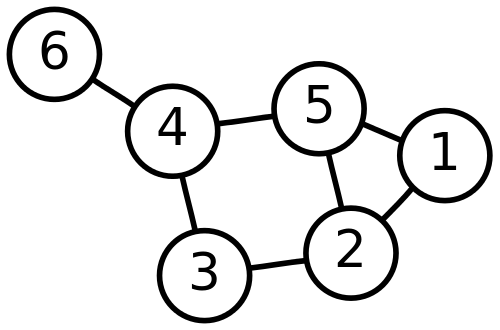
\includegraphics[width=0.85\linewidth]{img/6n-graph}
\column{.5\linewidth}
\[\left(
\begin{array}{cccccc}
0&1&0&0&1&0\\
1&0&1&0&1&0\\
0&1&0&1&0&0\\
0&0&1&0&1&1\\
1&1&0&1&0&0\\
0&0&0&1&0&0\\
\end{array}
\right)\]
\end{columns}
\end{frame}

\begin{frame}
\frametitle{Number of paths of length 2}
\begin{itemize}
\item Look at all possible intermediate nodes $k$
\item $\np2_{ij} = \textsf{sum}(\adj_{ik} \times \adj_{kj})$
\item $\adj_{ik}$ is line $i$ and $\adj_{kj}$ is column $j$
\end{itemize}

Example: number of paths from 2 to 4:
\[
\left(
\begin{array}{cccccc}
0&1&0&\mathbf{0}&1&0\\
\mathbf{1}&\mathbf{0}&\mathbf{1}&\mathbf{0}&\mathbf{1}&\mathbf{0}\\
0&1&0&\mathbf{1}&0&0\\
0&0&1&\mathbf{0}&1&1\\
1&1&0&\mathbf{1}&0&0\\
0&0&0&\mathbf{1}&0&0\\
\end{array}
\right)^2
=
\left(
\begin{array}{cccccc}
2&1&1&1&1&0\\
1&3&0&\mathbf{2}&1&0\\
1&0&2&0&2&1\\
1&2&0&3&0&0\\
1&1&2&0&3&1\\
0&0&1&0&1&1\\
\end{array}
\right)
\]
This is just matrix multiplication: $\np2 = \adj^2$
\end{frame}

\begin{frame}
\frametitle{Number of paths of length 3}
\begin{itemize}
\item We look at all the intermediate nodes
\item $\np3_{ij} = \textsf{sum}(\np2_{ik} \times \adj_{kj})$
\item $\np2_{ik}$ is line $i$ and $\adj_{kj}$ is column $j$
\end{itemize}

Example: number of paths from 1 to 4
\[
\underbrace{
\left(
\begin{array}{cccccc}
\mathbf{2}&\mathbf{1}&\mathbf{1}&\mathbf{1}&\mathbf{1}&\mathbf{0}\\
1&3&0&2&1&0\\
1&0&2&0&2&1\\
1&2&0&3&0&0\\
1&1&2&0&3&1\\
0&0&1&0&1&1\\
\end{array}
\right)
}_{\mbox{$\np2$}}
\ \underbrace{
\left(
\begin{array}{cccccc}
0&1&0&\mathbf{0}&1&0\\
1&0&1&\mathbf{0}&1&0\\
0&1&0&\mathbf{1}&0&0\\
0&0&1&\mathbf{0}&1&1\\
1&1&0&\mathbf{1}&0&0\\
0&0&0&\mathbf{1}&0&0\\
\end{array}
\right)
}_{\mbox{$\adj$}}
\rightarrow 2
\]
So $\np3 = \np2 \times \adj = \adj^2 \times \adj = \adj^3$
\end{frame}

\begin{frame}
\frametitle{Number of paths of any length}
\begin{itemize}
\item In general, the number of paths of length $n$ can be computed with $\adj^n$
\item So for $V$ nodes, we can get it in $O(V^3 \log n)$
\end{itemize}

~

Remarks:
\begin{itemize}
\item This also works with directed graphs (one-way edges)
\item This also works with multiple edges between two nodes (put the number in the matrix)
\item If you only want to know if there \emph{is a path or not}, you can do it in $O(V+E)$ for one source, or $O(V(V+E))$ for all pairs. (Fun exercise!)
\end{itemize}
\end{frame}

\section{Tortoise and hare}

\begin{frame}
\frametitle{Cycle finding problem}
\begin{itemize}
\item Finite set of states $S$, for example $\{1,\ldots,n\}$
\item Function $f: S \to S$ of transitions $x \mapsto f(x)$
\item Starting value: $x_0 \in S$
\end{itemize}

~

What is the first value repeated in this sequence?
\[ x_0,\ f(x_0),\ f(f(x_0)),\ f(f(f(x_0))), \ldots \]
\end{frame}

\begin{frame}
\frametitle{Cycle finding example}
Table of $f$:
\begin{center}
\begin{tabu}{c|ccccccccc}
$x$ &    1&2&3&4&5&6&7&8&9\\
\midrule
$f(x)$ & 8&6&1&7&1&4&5&5&2\\
\end{tabu}
\end{center}

~

Sequence for $x_0=9$:
\[
\underbrace{9,\ 2,\ 6,\ 4,\ 7}_\text{tail},
\ \underbrace{5,\ 1,\ 8}_\text{cycle},
\ \underbrace{5,\ 1,\ 8}_\text{cycle},
\ 5,\ 1,\ldots
\]

Problem: find the tail size and the cycle size
\end{frame}

\begin{frame}[fragile]
\frametitle{Cycle finding with map}
\begin{lstlisting}[frame=single]
pair<int,int> findCycle(int x)
{
    map<int,int> pos;
    
    // While x is a new value
    int i;
    for (i = 0; pos.find(x) == pos.end(); i++)
    {
        pos[x] = i; // Remember the position
        x = f(x);   // Move one step
    }
    return make_pair(pos[x], i - pos[x]);
}
\end{lstlisting}
\begin{itemize}
\item Time: $O(n \log n)$, or $O(n)$ with hashmap
\item Space: $O(n)$, that's a lot...
\end{itemize}
\end{frame}

\begin{frame}
\frametitle{Tortoise and hare 1: find match}
Keep two pointers: tortoise (slow) and hare ($2\,\times$\,faster)

~

Iterate until match:
\begin{center}
\begin{tabu}{rrrrrrrrrrrrrrr}
9&2&6&4&7&5&\textbf{1}&8&5&1&8&5&\textbf{1}&8&5\\
\midrule
%T\&H\\
&T&H\\
&&T&&H\\
&&&T&&&H\\
&&&&T&&&&H\\
&&&&&T&&&&&H\\
&&&&&&T&&&&&&H\\
\end{tabu}
\end{center}
The gap is a multiple of the cycle length
\end{frame}

\begin{frame}
\frametitle{Tortoise and hare 2: find tail}
Hare jumps to beginning, then they move at the same speed (the hare is tired by the jump)

~

Iterate until match:
\begin{center}
\begin{tabu}{rrrrrrrrrrrrrrr}
9&2&6&4&7&\textbf{5}&1&8&5&1&8&\textbf{5}&1&8&5\\
\midrule
H&&&&&&T\\
&H&&&&&&T\\
&&H&&&&&&T\\
&&&H&&&&&&T\\
&&&&H&&&&&&T\\
&&&&&H&&&&&&T\\
\end{tabu}
\end{center}
The number of steps is the tail length
\end{frame}

\begin{frame}
\frametitle{Tortoise and hare 3: find cycle}
Hare stops (\emph{really} tired) and tortoise continues

~

Iterate until next match:
\begin{center}
\begin{tabu}{rrrrrrrrrrrrrrr}
9&2&6&4&7&\textbf{5}&1&8&5&1&8&5&1&8&\textbf{5}\\
\midrule
&&&&&H&&&&&&T\\
&&&&&H&&&&&&&T\\
&&&&&H&&&&&&&&T\\
&&&&&H&&&&&&&&&T\\
\end{tabu}
\end{center}
The number of steps is the cycle length
\end{frame}

\begin{frame}[fragile]
\frametitle{Tortoise and hare: implementation}
\begin{lstlisting}[frame=single]
pair<int,int> findCycle(int x0)
{
    int t = x0, h = x0, tail = 0, cycle = 0;
    // Part 1: find a match
    do { t = f(t); h = f(f(h)); } while (t != h);
    // Part 2: find tail
    h = x0; // Rabbit jump
    while (t != h) { t = f(t); h = f(h); tail++; }
    // Part 3: find cycle
    do { t = f(t); cycle++; } while (t != h);
    return make_pair(tail, cycle);
}
\end{lstlisting}
\end{frame}

\end{document}
